%---------------------------------------------------------------------
\begin{frame}{Understanding health insurance plans}

    Sometimes soon, you will
    \begin{itemize}
        \item Choose a health plan or
        \item Choose between jobs with different benefits
    \end{itemize}
    $\implies$ Today's class should help you better understand these choices and your options.
    \vspace{3mm}

    We will talk primarily about two main dimensions of health insurance plans:
    \begin{itemize}
        \item Cost-sharing features of health plans
        \item Types of plans ``plan types''
    \end{itemize}
\end{frame}
%---------------------------------------------------------------------
\begin{frame}{}

    \begin{center}
        \Large \textcolor{maroon}{What does a health insurance plan look like?}
        \end{center}
\end{frame}
%---------------------------------------------------------------------
\begin{frame}{Vocabulary}

    \begin{itemize}
        \item \newbold{Premium}: Amount you pay each month (or each year) when enrolled in the plan.
        \pause
        \item \newbold{Out-of-pocket (OOP) cost}: Amount you pay ``out of your own pocket'' to get healthcare services. Your ``cost-sharing'' amount.
        \begin{itemize}
            \item Note that this is always zero if you consume zero healthcare services.
            \item It does not include the plan premium.
        \end{itemize}
        \pause
    
        \item \newbold{Total healthcare spending}: Your total amount of healthcare utilization.
        \begin{itemize}
            \item This is equal to the total dollars received by the healthcare providers that cared for you during the year.
            \item A portion of this amount is paid by you (your OOP cost) and the rest is paid by your insurer.
            \item[$\rightarrow$] \emph{OOP spending} + \emph{insurer spending} = \emph{total healthcare spending}
        \end{itemize}
    \end{itemize}
    
\end{frame}
%---------------------------------------------------------------------
\begin{frame}{Vocabulary}

    Plan cost-sharing features:
    \begin{itemize}
        \item \newbold{Deductible}: Amount you pay out-of-pocket before the plan pays anything.
        \item \newbold{Coinsurance}: Percent of healthcare bill you pay (after deductible is met).
        \item \newbold{Out-of-pocket max}: Maximum amount you will have to pay out-of-pocket in a year.
    \end{itemize}
    
\end{frame}
%---------------------------------------------------------------------
\begin{frame}{Example of a simple plan}

    Imagine you are offered this health insurance plan:
    \begin{itemize}
        \item Premium: \$1,000 (per year)
        \item Deductible: \$1,000
        \item Coinsurance: 20\%
        \item Out-of-pocket max: \$3,000
    \end{itemize}
    \pause
    \vspace{5mm} What would your out-of-pocket cost look like?
    
\end{frame}
%---------------------------------------------------------------------
\begin{frame}{Example of a plan: cost-sharing schedule}

    \centering
    \resizebox{0.7\textwidth}{!}{%
    \begin{tikzpicture}[>=Latex]
    
    \def\D{4.2}
    \def\M{9.2}
    \def\yD{3.2}
    \pgfmathsetmacro{\yMcalc}{\yD + 0.30*(\M-\D)}
    
    % Axes
    \draw[very thick,->] (0,0) -- (12,0);
    \draw[very thick,->] (0,0) -- (0,7.5);
    
    % Axis labels (FIXED)
    \node[below, font=\large, yshift = -18pt] at (6,0) {Dollars of health care expenses};
    \node[rotate=90, font=\large] at (-1.8,3.75) {Dollars of out-of-pocket expenses};
    
    % Vertical dashed lines
    \draw[dashed, thick] (\D,0) -- (\D,7.2);
    \draw[dashed, thick] (\M,0) -- (\M,7.2);
    
    % Labels on x-axis
    \node[below] at (\D,0) {\large 1,000};
    \node[below] at (\M,0) {\large max-OOP threshold};
    
    % OOP schedule
    \draw[very thick] (0,0) -- (\D,\yD);
    \draw[very thick] (\D,\yD) -- (\M,\yMcalc);
    \draw[very thick] (\M,\yMcalc) -- (12,\yMcalc);
    \draw[dashed, thick] (10.2,\yMcalc) -- (12,\yMcalc);
    
    % Slope annotations
    \node[rotate=36, yshift=7pt] at (2.2,1.9) {\large slope = 1};
    \node[rotate=17, yshift=5pt] at (6.8,4.2) {\large slope = 0.20};
    \node at (10.7,\yMcalc+0.35) {\large slope = 0};
    
    % Horizontal dashed line at OOP max = 3000
    \draw[dashed, gray, thick] (0,\yMcalc) -- (12,\yMcalc);
    \draw[gray, thick] (-0.15,\yMcalc) -- (0.15,\yMcalc);
    \node[left, gray, xshift=-4pt] at (0,\yMcalc) {\large 3{,}000};

    % Region braces
    \draw[decorate, decoration={brace, amplitude=6pt}]
        (0.6,6.0) -- (\D-0.25,6.0);
    \node[font=\large\itshape] at (\D/2,6.7) {deductible region};
    
    \draw[decorate, decoration={brace, amplitude=6pt}]
        (\D+0.25,6.0) -- (\M-0.25,6.0);
    \node[font=\large\itshape, align=center] at ({(\D+\M)/2},6.9)
        {20\% coinsurance\\region};
    
    \draw[decorate, decoration={brace, amplitude=6pt}]
        (\M+0.25,6.0) -- (11.6,6.0);
    \node[font=\large\itshape, align=center] at ({(\M+12)/2},6.9)
        {catastrophic \\care region};
    
    \end{tikzpicture}%
    }
\end{frame}
%---------------------------------------------------------------------
\begin{frame}{Example of a plan: cost-sharing schedule and premium}

    \centering
    \resizebox{0.7\textwidth}{!}{%
    \begin{tikzpicture}[>=Latex]
    
    \def\D{4.2}
    \def\M{9.2}
    \def\yD{3.2}
    
    % NOTE: your segment uses 0.30 here; change to 0.20 if you want 20% coinsurance
    \pgfmathsetmacro{\yMcalc}{\yD + 0.30*(\M-\D)}
    
    % Vertical shift corresponding to $1,000 (since $3,000 corresponds to yMcalc)
    \pgfmathsetmacro{\yShift}{\yMcalc/3}
    
    % Axes
    \draw[very thick,->] (0,0) -- (12,0);
    \draw[very thick,->] (0,0) -- (0,7.5);
    
    % Axis labels
    \node[below, font=\large, yshift=-18pt] at (6,0) {Dollars of health care expenses};
    \node[rotate=90, font=\large] at (-1.8,3.75) {Dollars of out-of-pocket expenses};
    
    % Vertical dashed lines
    \draw[dashed, thick] (\D,0) -- (\D,7.2);
    \draw[dashed, thick] (\M,0) -- (\M,7.2);
    
    % Labels on x-axis
    \node[below] at (\D,0) {\large 1,000};
    \node[below] at (\M,0) {\large max-OOP threshold};
    
    % OOP schedule (SHIFTED UP by yShift)
    \draw[very thick] (0,\yShift) -- (\D,\yD+\yShift);
    \draw[very thick] (\D,\yD+\yShift) -- (\M,\yMcalc+\yShift);
    \draw[very thick] (\M,\yMcalc+\yShift) -- (12,\yMcalc+\yShift);
    \draw[dashed, thick] (10.2,\yMcalc+\yShift) -- (12,\yMcalc+\yShift);
    
    % Slope annotations (shifted up so they stay attached to the lines)
    \node[rotate=36, yshift=7pt] at (2.2,1.9+\yShift) {\large slope = 1};
    \node[rotate=17, yshift=5pt] at (6.8,4.2+\yShift) {\large slope = 0.20};
    \node at (10.7,\yMcalc+\yShift+0.35) {\large slope = 0};
    
    % Horizontal dashed line at OOP max = 3000 (shifted up as well)
    \draw[dashed, gray, thick] (0,\yMcalc+\yShift) -- (12,\yMcalc+\yShift);
    \draw[gray, thick] (-0.15,\yMcalc+\yShift) -- (0.15,\yMcalc+\yShift);
    \node[left, gray, xshift=-4pt] at (0,\yMcalc+\yShift) {\large 4{,}000};
    
    % Tick/label at the new intercept = 1,000
    \draw[gray, thick] (-0.15,\yShift) -- (0.15,\yShift);
    \node[left, gray, xshift=-4pt] at (0,\yShift) {\large 1{,}000};
    
    % Region braces
    \def\braceYshift{1.1}  % adjust: 0.3 = small, 0.7 = larger
    \draw[decorate, decoration={brace, amplitude=6pt}]
        (0.6,6.0+\braceYshift) -- (\D-0.25,6.0+\braceYshift);
    \node[font=\large\itshape] at (\D/2,6.7+\braceYshift) {deductible region};
    
    \draw[decorate, decoration={brace, amplitude=6pt}]
        (\D+0.25,6.0+\braceYshift) -- (\M-0.25,6.0+\braceYshift);
    \node[font=\large\itshape, align=center] at ({(\D+\M)/2},6.9+\braceYshift)
        {20\% coinsurance\\region};
    
    \draw[decorate, decoration={brace, amplitude=6pt}]
        (\M+0.25,6.0+\braceYshift) -- (11.6,6.0+\braceYshift);
    \node[font=\large\itshape, align=center] at ({(\M+12)/2},6.9+\braceYshift)
        {catastrophic \\care region};
    
    \end{tikzpicture}%
    }
\end{frame}
%---------------------------------------------------------------------
% \begin{frame}{Example of a plan: cost-sharing schedule and premium}

%     \centering
%     \resizebox{0.7\textwidth}{!}{%
%     \begin{tikzpicture}[>=Latex]
    
%     \def\D{4.2}
%     \def\M{9.2}
%     \def\yD{3.2}
    
%     % NOTE: your segment uses 0.30 here; change to 0.20 if you want 20% coinsurance
%     \pgfmathsetmacro{\yMcalc}{\yD + 0.30*(\M-\D)}
    
%     % Vertical shift corresponding to $1,000 (since $3,000 corresponds to yMcalc)
%     \pgfmathsetmacro{\yShift}{\yMcalc/3}
    
%     % Axes
%     \draw[very thick,->] (0,0) -- (12,0);
%     \draw[very thick,->] (0,0) -- (0,7.5);
    
%     % Axis labels
%     \node[below, font=\large, yshift=-18pt] at (6,0) {Dollars of health care expenses};
%     \node[rotate=90, font=\large] at (-1.8,3.75) {Dollars of out-of-pocket expenses};
    
%     % Vertical dashed lines
%     \draw[dashed, thick] (\D,0) -- (\D,7.2);
%     \draw[dashed, thick] (\M,0) -- (\M,7.2);
    
%     % Labels on x-axis
%     \node[below] at (\D,0) {\large 1,000};
%     \node[below] at (\M,0) {\large max-OOP threshold};
    
%     % OOP schedule (SHIFTED UP by yShift)
%     \draw[very thick] (0,\yShift) -- (\D,\yD+\yShift);
%     \draw[very thick] (\D,\yD+\yShift) -- (\M,\yMcalc+\yShift);
%     \draw[very thick] (\M,\yMcalc+\yShift) -- (12,\yMcalc+\yShift);
%     \draw[dashed, thick] (10.2,\yMcalc+\yShift) -- (12,\yMcalc+\yShift);
    
%     % Slope annotations (shifted up so they stay attached to the lines)
%     \node[rotate=36, yshift=7pt] at (2.2,1.9+\yShift) {\large slope = 1};
%     \node[rotate=17, yshift=5pt] at (6.8,4.2+\yShift) {\large slope = 0.20};
%     \node at (10.7,\yMcalc+\yShift+0.35) {\large slope = 0};
    
%     % Horizontal dashed line at OOP max = 3000 (shifted up as well)
%     \draw[dashed, gray, thick] (0,\yMcalc+\yShift) -- (12,\yMcalc+\yShift);
%     \draw[gray, thick] (-0.15,\yMcalc+\yShift) -- (0.15,\yMcalc+\yShift);
%     \node[left, gray, xshift=-4pt] at (0,\yMcalc+\yShift) {\large 4{,}000};
    
%     % Tick/label at the new intercept = 1,000
%     \draw[gray, thick] (-0.15,\yShift) -- (0.15,\yShift);
%     \node[left, gray, xshift=-4pt] at (0,\yShift) {\large 1{,}000};
    
%     % Region braces
%     \def\braceYshift{1.1}  % adjust: 0.3 = small, 0.7 = larger
%     \draw[decorate, decoration={brace, amplitude=6pt}]
%         (0.6,6.0+\braceYshift) -- (\D-0.25,6.0+\braceYshift);
%     \node[font=\large\itshape] at (\D/2,6.7+\braceYshift) {deductible region};
    
%     \draw[decorate, decoration={brace, amplitude=6pt}]
%         (\D+0.25,6.0+\braceYshift) -- (\M-0.25,6.0+\braceYshift);
%     \node[font=\large\itshape, align=center] at ({(\D+\M)/2},6.9+\braceYshift)
%         {20\% coinsurance\\region};
    
%     \draw[decorate, decoration={brace, amplitude=6pt}]
%         (\M+0.25,6.0+\braceYshift) -- (11.6,6.0+\braceYshift);
%     \node[font=\large\itshape, align=center] at ({(\M+12)/2},6.9+\braceYshift)
%         {catastrophic \\care region};

%     % Reference line y = x
%     \draw[dashed, red, thick] (0,0) -- (7.5,7.5);
%     \node[red, rotate=45] at (2.2,2.6) {$y=x$};

%     \pgfmathsetmacro{\xIntersect}{
%     (\yShift + \yD - 0.20*\D)/0.8
%     }
%     % Intersection point with y = x
%     \filldraw[red] (\xIntersect+0.03,\xIntersect+0.03) circle (2.5pt);

%     % Dashed vertical line from intersection to x-axis
%     \draw[dashed, gray]
%     (\xIntersect,\xIntersect) -- (\xIntersect,0);

%     % Red arrow starting midway down the dashed line
%     \pgfmathsetmacro{\yMid}{\xIntersect/2}

%     \draw[->, blue, thick]
%     (\xIntersect+0.2,\xIntersect) -- (\xIntersect+3.6,\xIntersect);

%     % Left arrow
%     % \draw[->, blue, thick]
%     % (\xIntersect,\yMid) -- (\xIntersect-1.6,\yMid);

%     % \node[blue, below]
%     % at (\xIntersect+1.5,\yMid) {\large yes};
%     % \node[blue, below]
%     % at (\xIntersect-0.8,\yMid) {\large no};


%     \end{tikzpicture}%
%     }
% \end{frame}
%---------------------------------------------------------------------
\begin{frame}{Actuarial value of a plan}

    \newbold{Actuarial value (AV)} of a plan: the percentage of total costs that a plan will cover \textit{on average}
    \begin{equation*}
        AV = \frac{\mathbb{E}[\text{Insurer Payments}]}{\mathbb{E}[\text{Total Spending}]}
    \end{equation*}
    \begin{itemize}
        \item Example: A plan with AV = 80\% means that, on average, the plan pays for 80\% of total healthcare spending and the enrollee pays 20\%.
    \end{itemize}
    \vspace{5mm}
    Note: AV \textbf{does not} include the premium
    
\end{frame}
%---------------------------------------------------------------------
\begin{frame}{Actuarial value of a plan}

    \newbold{Actuarial value (AV)} of a plan: the percentage of total costs that a plan will cover \textit{on average}
    \begin{equation*}
        AV = \frac{\mathbb{E}[\text{Insurer Payments}]}{\mathbb{E}[\text{Total Spending}]}
    \end{equation*}

    Questions:
    \begin{itemize}
        \item {\color{gray} Do you expect AVs and premiums to be correlated across plans and across insurers? Why?}
        \only<2|3>{{\color{red} Yes, positively correlated. Varies with the generosity of the plan, which influences the premium too.}}
        \item {\color{gray} What is the AV for a plan with no deductible, a constant coinsurance rate $c$, and no out-of-pocket maximum?}
        \only<3>{{\color{red} AV = 1 - c}}
    \end{itemize}
    
\end{frame}
%---------------------------------------------------------------------
\begin{frame}{Expected medical costs covered}

    % add figure from health insurance notes
    \begin{center}
        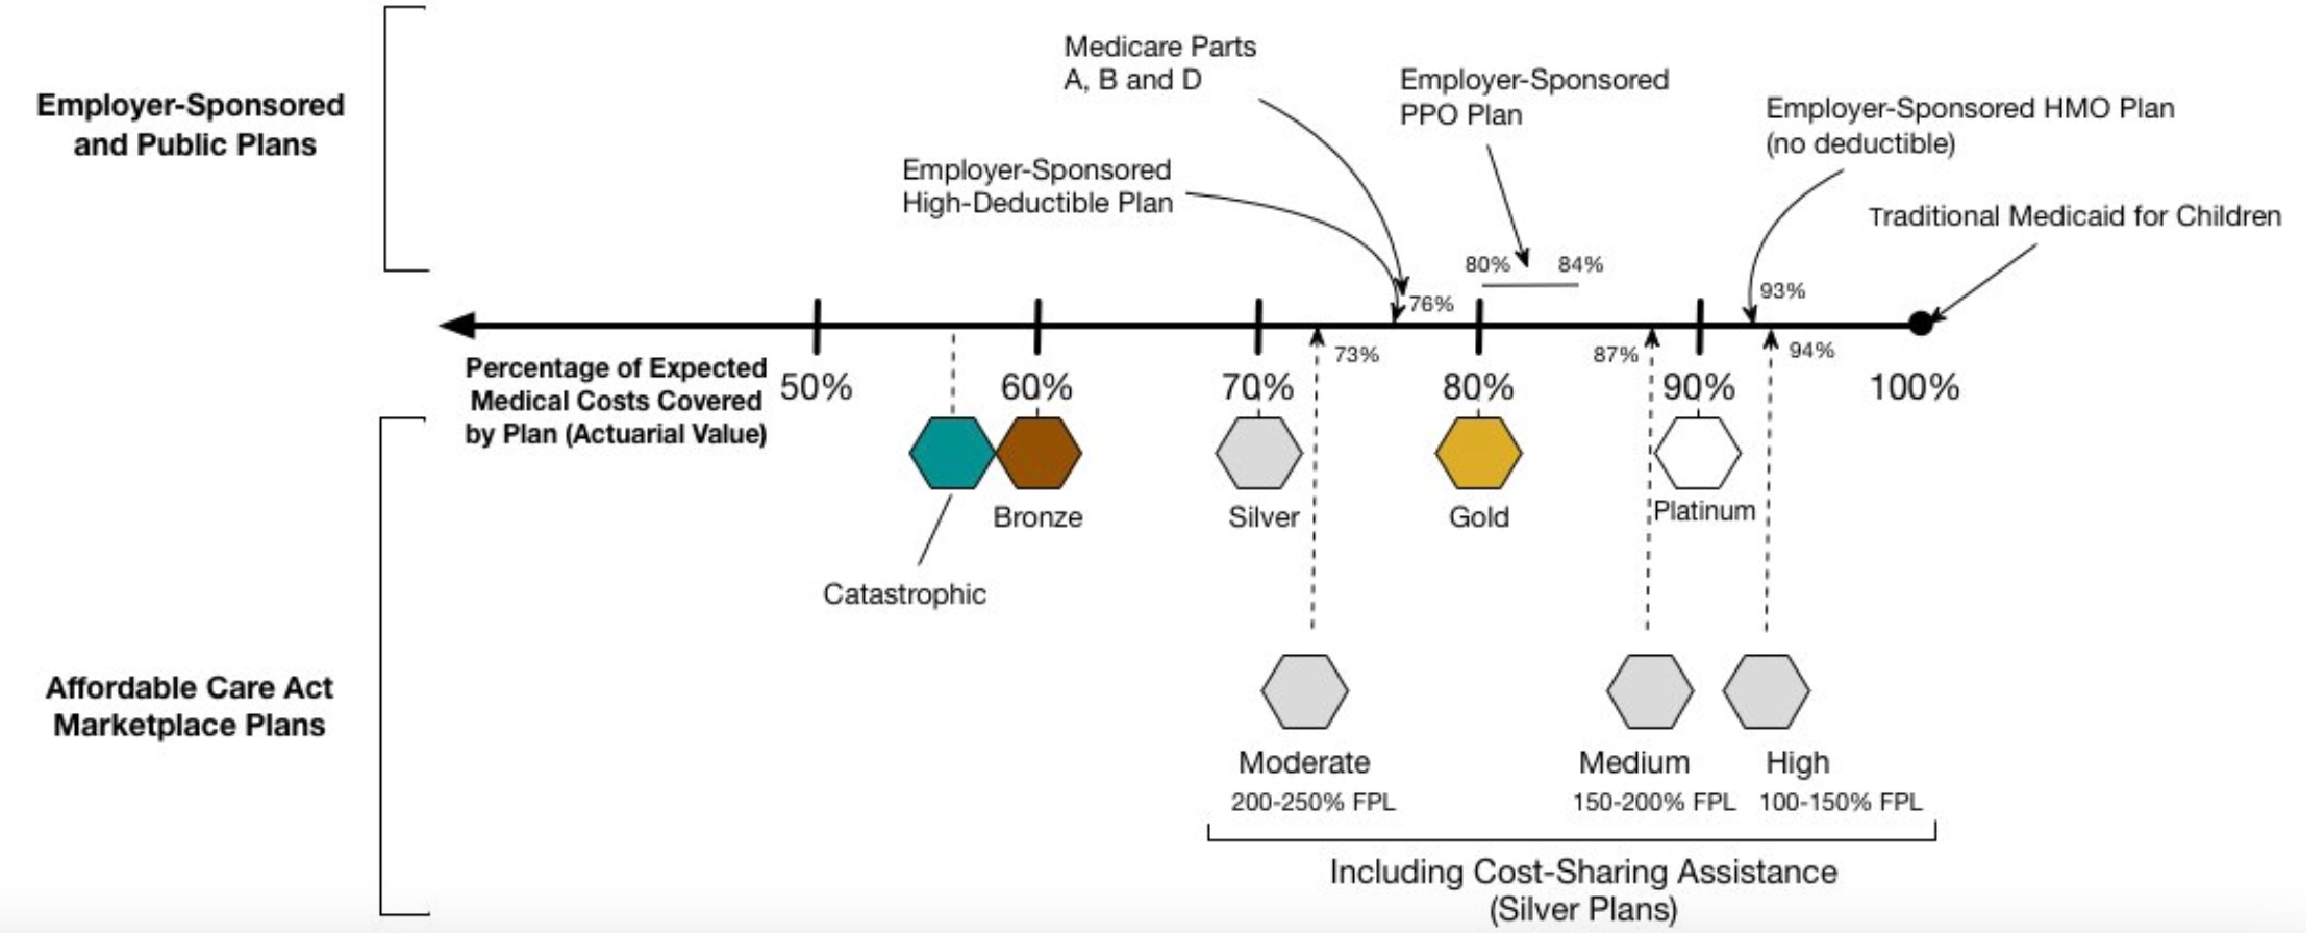
\includegraphics[width=0.95\textwidth]{input/plans_coverage_ratings.pdf}
    \end{center}
    {\small 
    Source: \url{https://www.twitter.com/johngraves9/status/818933041808674816}}
    
\end{frame}
%---------------------------------------------------------------------
\begin{frame}{What are the ``types'' of plans?}

    \begin{itemize}
        \item \textbf{HMO – Health Maintenance Organization}
        \begin{itemize}
            \item Gatekeeping (need referral from PCP for specialist care)
            \item Typically, lower premiums and lower out-of-pocket costs
            \item Primarily uses gatekeeping (rather than cost-sharing) to limit moral hazard
            \item Limited networks: no coverage if you see Out-Of-Network providers
        \end{itemize}
    
        \vspace{0.3cm}
    
        \item \textbf{PPO – Preferred Provider Organization}
        \begin{itemize}
            \item Usually, no referrals needed to see specialist
            \item Higher premiums than HMOs and typically higher cost-sharing
            \item Primarily uses cost-sharing (rather than gatekeeping) to limit moral hazard
            \item Wider networks:
            \begin{itemize}
                \item Typically, a larger set of In-Network providers than HMOs
                \item Also still get some coverage if you go Out-Of-Network
            \end{itemize}
        \end{itemize}
    \end{itemize}
\end{frame}
%---------------------------------------------------------------------
\begin{frame}{What are the ``types'' of plans?}

    \begin{itemize}
        \item \textbf{HDHP – High Deductible Health Plans}
        \begin{itemize}
            \item Can make pre-tax contributions to HSA (Health Savings Account)
            \item Least expensive premium
            \item Primarily uses cost-sharing (rather than gatekeeping) to limit moral hazard
            \item May still have provider network (like a PPO), or may just have no network restrictions
        \end{itemize}
    \end{itemize}
\end{frame}
%---------------------------------------------------------------------
\begin{frame}{}
    \vspace{2mm}
    \begin{center}
        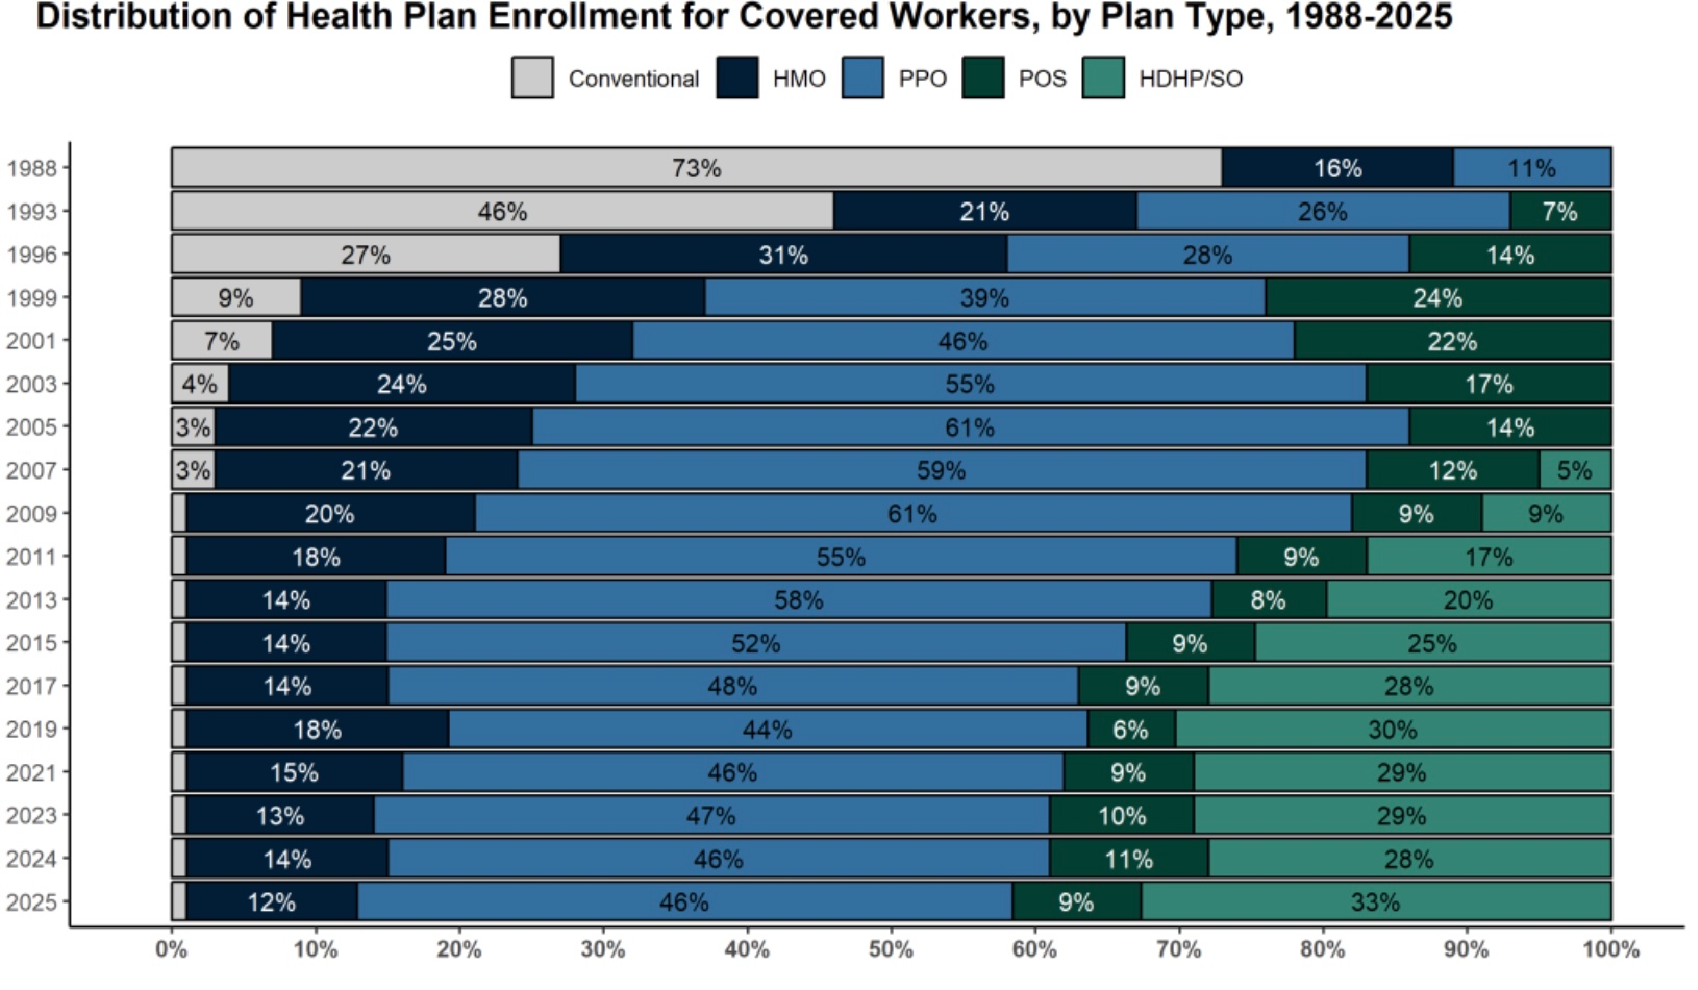
\includegraphics[width=0.9\textwidth]{input/ESI_plan_type_overtime_KFF.pdf}
    \end{center}
    {\small 
    Source: \href{https://www.kff.org/health-costs/2025-employer-health-benefits-survey}{KFF website}}
    
\end{frame}
%---------------------------------------------------------------------
\begin{frame}{Definitions}

    {\scriptsize
    \begin{itemize}
        \item \textbf{HMO} is a health maintenance organization. The survey defines an HMO
        as a plan that does not cover non-emergency out-of-network services.
    
        \item \textbf{PPO} is a preferred provider organization. The survey defines PPOs as
        plans that have lower cost sharing for in-network provider services, and do not
        require a primary care gatekeeper to screen for specialist and hospital visits.
    
        \item \textbf{POS} is a point-of-service plan. The survey defines POS plans as those
        that have lower cost sharing for in-network provider services, but do require a
        primary care gatekeeper to screen for specialist and hospital visits.
    
        \item \textbf{HDHP/SO} is a high-deductible health plan with a savings option such as
        an HRA or HSA. HDHP/SOs are treated as a distinct plan type even if the plan would
        otherwise be considered a PPO, HMO, POS plan, or indemnity plan. These plans have a
        deductible of at least \$1{,}000 for single coverage and \$2{,}000 for family
        coverage and are offered with an HRA, or are HSA-qualified. See Section~8 for more
        information on HDHP/SOs.
    
        \item \textbf{Conventional/Indemnity}: The survey defines conventional or indemnity
        plans as those that have no preferred provider networks and the same cost sharing
        regardless of physician or hospital.
    \end{itemize}
    } 
   
\end{frame}
%---------------------------------------------------------------------
\begin{frame}{}

    \begin{center}
        \Large \textcolor{maroon}{Let's practice what we have learnt}
        \end{center}
\end{frame}
%---------------------------------------------------------------------
\begin{frame}{Understanding a proposed health insurance plan}

    Plan A with the following parameters:
    \begin{itemize}
        \item Premium: \$1,200 per year
        \item Deductible: \$1,000
        \item Coinsurance: 10\%
        \item Out-of-pocket max: \$2,500
    \end{itemize}
    \vspace{3mm}

    Questions:
    \begin{enumerate}
        \only<1>{\item[1.] Draw the relationship between out-of-pocket costs (y-axis) and total health care expenses (x-axis) for this plan. \textit{Note: do not include the premium in this graph.}}
        \only<2>{\item[2.] Someone who has this plan breaks their arm and generate \$400 in medical bills. That's their only contact with the medical system that year. How much do they pay out of pocket for this encounter?}
        \only<3>{\item[3.] This person is later told that they need an MRI to assess whether there is any damage to ther ligaments. The MRI generates another \$3,000 in medical bills. 
        This happens the same year as teh broken arm. How much do they pay out of pocket for the MRI (not including that broken arm bill, which was separate)?}
        \only<4>{\item[4.] Another person on this plan takes Capaxone each month to treat their multiple sclerosis. The drug costs \$1,000 per month.
        In addition, this person anticipates \$8,000 in various medical costs this same year.
        How much should they anticipate to spend out of pocket this year when enrolled in this plan?
        If things get much worse than anticipated for this person,
        should they worry that their out of pocket costs would be higher?}
    \end{enumerate}


\end{frame}
%---------------------------------------------------------------------
\begin{frame}{Comparing two plans when minimizing own healthcare spending}

    Two plans are proposed
    \begin{enumerate}
        \item Plan A: premium \$1,200 per year, deductible \$1,000, coinsurance 10\%, out-of-pocket max \$2,500
        \item Plan B: premium \$0 per year, deductible \$2,000, coinsurance 14.3\%, out-of-pocket max \$4,000
    \end{enumerate}
    \vspace{3mm}

    Questions:
    \begin{enumerate}
        \only<1>{\item[1.] Draw the relationship between total consumer-paid expenses (premium + out-of-pocket costs) (y-axis) and total health care expenses (x-axis) for these two plans.}
        \only<2>{\item[2.] Which plan minimizes total consumer-paid expenses for someone who expects to have \$3,000 in total health care expenses this year?}
        \only<3>{\item[3.] Which plan minimizes total consumer-paid expenses for someone who expects to have \$17,000 in total health care expenses this year?}
        \only<4>{\item[4.] At what level of total healthcare spending does plan A becomes better than plan B in terms of minimizing total consumer-paid expenses?}
    \end{enumerate}


\end{frame}
%---------------------------------------------------------------------
\begin{frame}{Buying health insurance}

    The consumer has \$20,000 in income and her utility function is $u(x) = \sqrt{x}$.\\
    She faces health risks such that
    \begin{itemize}
        \item She has a 50\% chance of having no medical expenses
        \item She has a 40\% chance of having \$1,000 in medical expenses (mild illness)
        \item She has a 10\% chance of having \$10,000 in medical expenses (severe illness)
    \end{itemize}
    \vspace{3mm}

    She is considering buying a health insurance plan with
    \begin{itemize}
        \item A premium of \$1,000
        \item A deductible of \$500
        \item A coinsurance rate of 20\%
    \end{itemize}

\end{frame}
%---------------------------------------------------------------------
\begin{frame}{Buying health insurance}

    Questions:
    \begin{enumerate}
        \item What is the consumer's expected out-of-pocket cost when uninsured?
        \item What is the expected cost to the insurer?
        \item What is the expected profit to the insurer?
        \item What would be the actuarially fair price for this insurance plan?\\
        \textit{Hint: the actuarially fair price is the premium that would give the insurer zero expected profit.}
        \item Does the consumer prefer to remain uninsured or to buy this insurance plan?
        \item What is the maximum premium the consumer would be willing to pay for this insurance plan?
    \end{enumerate}

\end{frame}
%---------------------------------------------------------------------
\begin{frame}{}
    \begin{center}
    \Large \textcolor{maroon}{Wrapping up}
    \end{center}

\end{frame}
%---------------------------------------------------------------------
\begin{frame}{What we covered today}
        \begin{itemize}
        \item Understanding an insurance plan
        \begin{itemize}
            \item Cost-sharing features of plans: premium, deductible, coinsurance, out-of-pocket max
            \item ``Types of plans'': HMO, PPO, HDHP
        \end{itemize}
        \item Demand for insurance\\
        {\small (willingness to pay, actuarially fair price, expected profit for insurer)}
    \end{itemize}
\end{frame}
%---------------------------------------------------------------------
\begin{frame}{To next class}
    \begin{itemize}
        \item \newbold{TO DO}
        \begin{enumerate}
            \item \newbold{Mandatory reading}: RAND Research Brief [reading 1]\\
            $\implies$ \textbf{We will discuss in class}
            \item \newbold{Problem set 2} due \newbold{next week}:\\
            by Thursday, Feb. 12th at 9:30am
            \item Review this class and past material $\implies$ \textit{questions on it?}
        \end{enumerate}
        \vspace{5mm}

        \item Program for next class
        \begin{itemize}
            \item Moral hazard
        \end{itemize}
    \end{itemize}
\end{frame}
%---------------------------------------------------------------------